\documentclass[12pt,oneside]{article}
\usepackage[paperheight=26cm,paperwidth=18.4cm]{geometry}
%\usepackage[paperwidth=9.2cm, paperheight=12.4cm, width=9cm, height=12cm,top=0.2cm,bottom=0.4cm,left=0.2cm,right=0.2cm,foot=0cm, nohead,nofoot]{geometry}
%\geometry{left=1cm,right=1cm,top=2cm,bottom=2cm}
\usepackage{anysize}
\papersize{26cm}{18.4cm}
\marginsize{1.5cm}{2.1cm}{2cm}{2cm} 
%\marginsize{1cm}{1cm}{1cm}{1cm} 

%\usepackage[utf8]{inputenc}
%\usepackage[T1]{fontenc}
\usepackage{fixltx2e}
\usepackage{graphicx}
\usepackage{longtable}
\usepackage{float}
\usepackage{wrapfig}
\usepackage{soul}
\usepackage{textcomp}
\usepackage{marvosym}
%\usepackage{wasysym}
\usepackage{latexsym}
\usepackage{amssymb}
%\usepackage{hyperref}
\tolerance=1000
\usepackage{etex}
\usepackage{amsmath}
\usepackage[usenames]{color}
\usepackage{pstricks}
\usepackage{pgfplots}
\usepackage{tikz}
\usepackage[europeanresistors,americaninductors]{circuitikz}
\usepackage{colortbl}
\usepackage{yfonts}
\usetikzlibrary{shapes,arrows,matrix}
\usetikzlibrary{positioning}
\usetikzlibrary{intersections}
\usetikzlibrary{calc,patterns,decorations.pathmorphing,decorations.markings}
\usepackage[BoldFont,SlantFont,CJKchecksingle]{xeCJK}
\usepackage{CJKnumb}
\setCJKmonofont{Evermore Kai}
\setCJKmainfont[BoldFont=Evermore Hei]{Evermore Song}
\setCJKfamilyfont{hei}{Evermore Hei}
%\usepackage{CJKnumb}
%\xeCJKsetup{CJKglue=\hspace{0pt plus .08 \baselineskip }}
\usepackage{pst-node}
\usepackage{pst-plot}
\psset{unit=5mm}
%\pdfcompresslevel=9
\DeclareGraphicsExtensions{.jpg,.pdf,.mps,.png}

%\usepackage{CJK,CJKnumb}
\usepackage{listings}
\usepackage{tabularx}
\usepackage{longtable}
\usepackage{indentfirst}                % 首行缩进宏包
\usepackage{color}                      % 支持彩色
\usepackage{listings}                   % 源代码宏包
\usepackage[perpage,symbol]{footmisc}   % 脚注控制
\usepackage{lastpage}                   % 自动记录总页数宏包,计数器为LastPage
\usepackage{fancyhdr}                   % fancyhdr宏包 页眉和页脚的相关定义
\pagestyle{empty}
\topmargin -5mm \oddsidemargin -10mm \evensidemargin -10mm \textwidth 150mm \textheight 200mm
\headsep 1em
\pagestyle{fancyplain}                  % 要在\usepackage{pageno}之前,不然页眉有一条黑线去不掉
%\usepackage{pageno}                     % 章首页的页眉处理, 可以改为自己想要的形式 


\renewcommand{\baselinestretch}{1.5}
\allowdisplaybreaks


%----------------------------------页眉页脚---------------------------------------
%\pagestyle{fancyplain}
\renewcommand{\headrulewidth}{0pt}
\fancyhf[C]{西北工业大学命题专用纸}
\fancyfoot[C]%[RE][LO]
{ \hfill \\
教务处印制\hfill 共\pageref{LastPage}页\quad 第\thepage 页}

\lfoot{\setlength{\unitlength}{1mm}
\begin{picture}(0,0)\linethickness{0.4mm}
\put(77,109){\makebox(0,0){\framebox(160,210){}}}
\end{picture}}
%---------------------------------------------------------------------------------


\begin{document}



%---------------------------------------源代码------------------------------------------------
\lstset{xleftmargin=1em,xrightmargin=1em}
\lstset{commentstyle=\textit,keywordstyle=\textbf,breaklines=true,columns=flexible,mathescape=true}
\lstdefinestyle{numbers}{numbers=left,stepnumber=1,numberstyle=\small,numbersep=1em}
\lstset{language=C++}
  \lstset{%
numbers=left,stepnumber=1,numberstyle=\tiny,
  %basicstyle=\footnotesize\ttfamily,
  basicstyle=\ttfamily,
  commentstyle=\textit,
  keywordstyle=\textbf,
  identifierstyle=\slshape,
  stringstyle=\small,
  %stringstyle=\color{orange},
  breaklines=true,
%    escapechar=\#,
    emphstyle=\bfseries\color{red}
}
\renewcommand{\lstlistingname}{程序}

%\CJKcaption{GB}
%\CJKcaption{gb_452}
%\CJKtilde \CJKindent

\newcounter{question}
\usecounter{question}
\setcounter{question}{1}
\newcommand{\question}{{\flushleft\CJKnumber{\arabic{question}}、}\stepcounter{question}}



%--------------------------------------首页页眉页脚---------------------------------------------
\fancypagestyle{plain}{%
\fancyhf{} % clear all header and footer fields
\renewcommand{\headrulewidth}{0pt}
\renewcommand{\footrulewidth}{0pt}
\fancyfoot[C]%[RE][LO]
{
\renewcommand{\baselinestretch}{1.0}
\begin{tabular}{ll} 
 注: &  命题纸上一般不留答题位置,试题请用小四、宋体打印且不出框。\\
% & 2. 命题教师和审题教师姓名应在试卷存档时填写。\hspace{3em} 共\pageref{LastPage}页 第\thepage页 
 &  \hspace{25em} 共\pageref{LastPage}页 第\thepage 页 
\end{tabular}
}
\lfoot{\setlength{\unitlength}{1mm}
\begin{picture}(0,0)\linethickness{0.4mm}
\put(77,52){\makebox(0,0){\framebox(160,88.5){}}}
\put(-3,85.5){\line(1,0){160}}
\put(0,89){\raisebox{0ex}[4ex][2ex]{考生班级}\  \vline \hspace{8em}\hfill \vline\ 学\hspace{1em}号\ \vline \hspace{10em}\hfill \vline\ 姓\hspace{1em}名\ \vline\hfill  \hspace{6eM} }
\end{picture}}}
\thispagestyle{plain}
%------------------------------------------------------------------------------------------------
\setlength{\unitlength}{1ex}
\begin{center}

\begin{minipage}{84ex}
\parbox{84ex}{\CJKfamily{hei}
\center{诚信保证} \\ \vspace{-2ex}
\flushleft
\hspace{2eM}本人知晓我校考场规则和违纪处分条例的有关规定,保证遵守考场规则,诚实做人。\hfill 本人签字:\underline{\hspace{4eM}}\\ \vspace{1ex}}
\end{minipage}

\begin{picture}(0,0)

\put(0,7){\makebox(0,0){\dashbox(92,14){}
}}
\end{picture}

\end{center}

%\large
\noindent 编号:\underline {\hspace{4eM}}


%\vspace{-6ex}

\begin{center}
\textbf{ \fontsize{18pt}{\baselineskip}\selectfont{西北工业大学考试试题(卷)}}\\
2018-2019 学年 秋 学期
\end{center}

{
\flushleft

\begin{tabular}{lll}
开课学院 \underline {\hspace{1em} 航天学院\hspace{1em} }& 课程\underline {\hspace{1em} 自动控制理论1\hspace{1em} }& 学时\underline {\hspace{1em} 48\hspace{1em} }\\
考试日期\underline {\hspace{6eM} }& 考试时间\underline {\hspace{1em} 2\hspace{1em} }小时 & 考试形式
$\left(\begin{array}{c}
\mbox{开}\\
\mbox{闭}
\end{array} \right)$
$\left(\begin{array}{*{10}c}
 \mbox{A} \\
 \mbox{B} 
\end{array} \right)$卷 
\end{tabular}
}

{
\center
%\renewcommand{\tabcolsep}{6pt}
\renewcommand{\tabcolsep}{1.2em}
\begin{tabular}{|c|c|c|c|c|c|c|c|c|c|} 
\hline
题号 & 一 & 二 & 三 & 四 & 五 & 六 & 七 & 八 & 总分 \\
\hline
得分 &    &    &    &    &    &    &    &    & \\
\hline 
\end{tabular}
}
\begin{tabular}{c}
\ \\
\ 
\end{tabular}
%\begin{minipage}{170mm}
%\ \raisebox{0ex}[4ex][2ex]{考生班级}\  \vline   \hfill \vline\ 学\hspace{1em}号\ \vline\hfill  \vline\ 姓\hspace{1em}名\ \vline\hfill  \hspace{6eM} \\
%\vskip -2.3ex \hrule
%\end{minipage}
\newcommand{\onlytest}[1]{#1}
\newcommand{\onlyanswer}[1]{}
%-----------------内容放在这里--------------------------


\question(20分)已知控制系统结构图如下所示,已知 $G(s)=\frac{1}{s+1},G_c(s)=1$ 。 若 $G_r(s)=\frac{k_1 s+k_2}{s+1},r(t)=t,(t>0)$ , 是否存在 $k_1,k_2$ 使稳态误差为零?
若$G_r(s)=Ae^{-\theta s},r(t)=sin(t),(t>0)$ 是否存在 $A,\theta,(\theta\in(0,2\pi))$ 使系统稳态输出 $c(t)=sin(t)$ ?


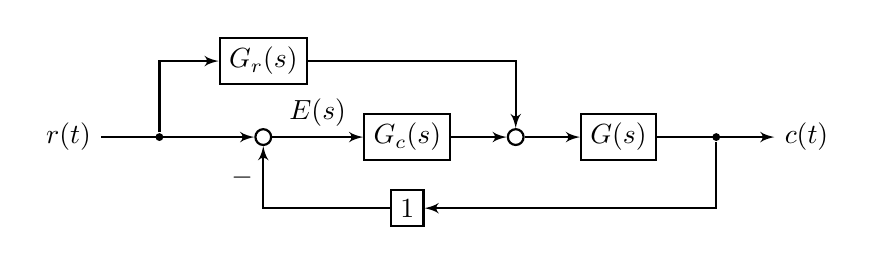
\begin{tikzpicture}[node distance=3em,auto,>=latex', thick]
%\path[use as bounding box] (-1,0) rectangle (10,-2); 
\tikzstyle{block} = [draw,rectangle,thick,minimum height=1em,minimum width=1em]
\tikzstyle{sum} = [draw,circle,inner sep=0mm,minimum size=2mm]
\tikzstyle{branch} = [circle,fill,inner sep=0pt,minimum size=1mm]
\tikzstyle{connector} = [->,thick]

\def\r{\node(r){$r(t)$};}
\def\b(#1){\node[branch](b#1){};}
\def\p(#1){\node[sum](p#1){};}
\def\gc{\node[block](gc){$G_c(s)$};}
\def\gr{\node[block](gr){$G_r(s)$};}
\def\gp{\node[block](gp){$G(s)$};}
\def\g(#1){\node[block](g#1){$1$};}
\def\c{\node(c){$c(t)$};}

\matrix[ampersand replacement=\&, row sep=1em, column sep=2em]{
	\&         \&   \gr  \\
	\r  \&   \b(r)  \& \p(e)  \& \gc \& \p(r) \& \gp \& \b(c)  \& \c  \\
	\&         \&         \& \g(h)    \\
};
\draw [connector](r) -- (pe) ; 
\draw [connector](br) |- (gr) ; 
\draw [connector](gr) -| (pr) ; 
\draw [connector](pe) -- node[midway]{$E(s)$} (gc) ; 
\draw [connector](gc) -- (pr) ; 
\draw [connector](pr) -- (gp) ; 
\draw [connector](gp) -- (c) ; 
\draw [connector](bc) |- (gh) ; 
\draw [connector](gh) -| node[near end , left]{$-$} (pe) ; 
\end{tikzpicture} 

\onlyanswer
{
	答:当 $G_r(s)=\frac{k_1 s+k_2}{s+1},r(t)=t,(t>0)$ 时,得:
	\begin{align*}
	\frac{E(s)}{R(s)} &= (1-\frac{k_1s+k_2}{s+1}\cdot\frac{1}{s+1})\frac{1}{1+\frac{1}{s+1}} \\
	&=\frac{(s+1)^2-(k_1s+k_2)}{(s+2)(s+1)} \\
	&=\frac{s^2+(2-k_1)s+(1-k_2)}{(s+2)(s+1)} \\
	\end{align*}
	所以,当 $k_1=2,k_2=1$ 时,
	\begin{align*}
	E(s) &=\frac{s^2+(2-k_1)s+(1-k_2)}{(s+2)(s+1)}\cdot R(s) \\
	&=\frac{s^2}{(s+2)(s+1)}\cdot \frac{1}{s^2} \\
	&=\frac{1}{(s+2)(s+1)} \\
	e_{ss} &= \lim_{s\rightarrow 0} sE(s) \\
	&= 0
	\end{align*}
	
	当 $G_r(s)=Ae^{-\theta s},r(t)=sin(t),(t>0)$ 时:
	\begin{align*}
	G(j\omega) &=\frac{1}{j\omega+1} \\
	G_r(j\omega) &=Ae^{-j\theta\omega} \\
	\frac{C(j\omega)}{R(j\omega)} &= \frac{G(j\omega)+G_r(j\omega)G(j\omega)}{1+G(j\omega)} \\
	&=\frac{1+Ae^{-j\theta\omega}}{2+j\omega}
	\end{align*}
	
	稳态时,
	\begin{align*}
	\left.\frac{C(j\omega)}{R(j\omega)}\right|_{\omega=1} &=\left.\frac{1+Ae^{-j\theta\omega}}{2+j\omega}\right|_{\omega=1} \\
	&=\frac{1+Ae^{-j\theta}}{2+j} \\
	&=1 
	\end{align*}
	得:
	\begin{align*}
	A &=\sqrt{2} \\
	\theta &=2n\pi-\frac{\pi}{4}\\
	&=\frac{7\pi}{4}
	\end{align*}
}

\onlytest{\newpage}

\question(20分)单位负反馈控制系统开环传递函数,
$$G(s)=\frac{20}{s(s+1)(s+5)}$$
串联校正网络:
$$G_c(s)=k\cdot\frac{aT_a s+1}{T_a s+1}$$
能否调整$k,a,T_a$使校正后系统截止频率保持不变,同时使相角裕度提高 $60^\circ$ 。

\onlyanswer
{
	答:
	\begin{align*}
	\phi_m &=\arcsin\frac{a-1}{a+1}\\
	&= 60^\circ \\
	a &=\frac{2+\sqrt{3}}{2-\sqrt{3}}\\
	\omega_c &=2=\omega_m\\
	&=\frac{1}{T_a\sqrt{a}}\\
	T_a &=\frac{1}{2}\sqrt{\frac{2-\sqrt{3}}{2+\sqrt{3}}}\\
	k &=\frac{1}{\sqrt{a}}\\
	&=\sqrt{\frac{2-\sqrt{3}}{2+\sqrt{3}}}
	\end{align*}
}



\question(20分){已知控制系统结构图如下所示。当$T_y=T,r(t)=t,(t>0)$时求系统稳态误差;当 $T_y=\frac{T}{2},R(z)=1$ 时,求 $Y(z)$ 。
	
	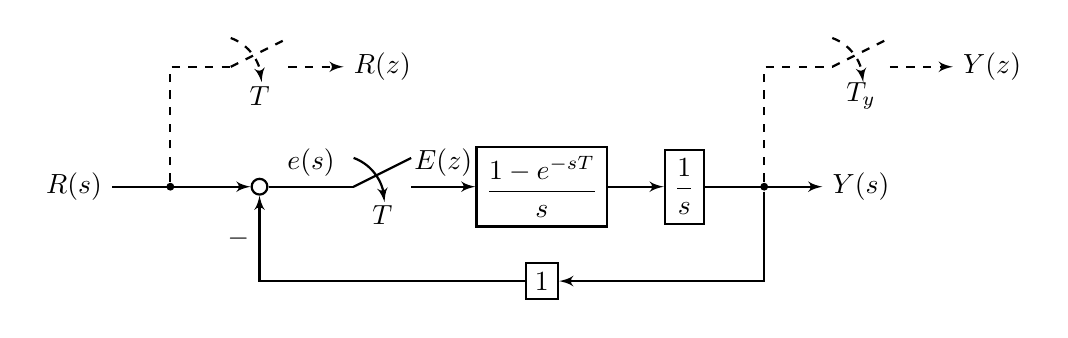
\begin{tikzpicture}[node distance=3em,auto,>=latex', thick]
	%\path[use as bounding box] (-1,0) rectangle (10,-2); 
	\tikzstyle{block} = [draw,rectangle,thick,minimum height=1em,minimum width=1em]
	\tikzstyle{sum} = [draw,circle,inner sep=0mm,minimum size=2mm]
	\tikzstyle{branch} = [circle,fill,inner sep=0pt,minimum size=1mm]
	\tikzstyle{connector} = [->,thick]
	
	\def\r{\node(r){$R(s)$};}
	\def\rd{\node(rd){$R(z)$};}
	\def\b(#1){\node[branch](b#1){};}
	\def\p(#1){\node[sum](p#1){};}
	\def\s(#1){\path[->] node[minimum size=2em] (s#1) {}; \draw (s#1.west)--(s#1.north east);\draw[->] (s#1.north west) arc (70:0:1.7em);\draw (s#1.south) node {$T$};}
	\def\sd(#1){\path[->] node[minimum size=2em] (sd#1) {}; \draw[dashed] (sd#1.west)--(sd#1.north east);\draw[dashed,->] (sd#1.north west) arc (70:0:1.7em);\draw[dashed] (sd#1.south) node {$T$};}
	\def\sdc(#1){\path[->] node[minimum size=2em] (sdc#1) {}; \draw[dashed] (sdc#1.west)--(sdc#1.north east);\draw[dashed,->] (sdc#1.north west) arc (70:0:1.7em);\draw[dashed] (sdc#1.south) node {$T_y$};}
	\def\ga{\node[block](g1){$\dfrac{1-e^{-sT}}{s}$};}
	\def\gb{\node[block](g2){$\dfrac{1}{s}$};}
	\def\g(#1){\node[block](g#1){$1$};}
	\def\c{\node(c){$Y(s)$};}
	\def\cd{\node(cd){$Y(z)$};}
	
	\matrix[ampersand replacement=\&, row sep=1em, column sep=2em]{
		\&         \& \sd(r)  \& \rd      \&  \&     \&          \&  \sdc(c)  \& \cd \\
		\r  \& \b(r)   \& \p(e)   \& \s(e) \& \ga \& \gb \&  \b(c)   \&  \c \\
		\&         \&         \&       \& \g(h) \\
	};
	\draw [connector](r) -- (pe) ; 
	\draw [dashed](br)  |- (sdr) ; 
	\draw [connector,dashed](sdr) -- (rd) ; 
	\path[](pe) edge node[midway] {$e(s)$} (se) ; 
	\draw [connector] (se) -- node[midway] {$E(z)$} (g1); 
	\draw [connector] (g1) -- node[midway] {$   $} (g2); 
	\draw [connector] (g2)-- (c); 
	\draw [dashed](bc)  |- (sdcc) ; 
	\draw [connector,dashed](sdcc) -- (cd) ; 
	\draw [connector](bc)  |- (gh) ; 
	\draw [connector](gh) -|  node[near end,left]{$-$} (pe) ; 
	\end{tikzpicture} 
	
	
	常见 $Z$ 变换表:
	$$
	\begin{array}{ccc}
	f(t)     &   F(s)  &  F(Z)   \\ 
	\delta(t)   &   1      &  1    \\  
	1(t)         &   \frac{1}{s} &  \frac{1}{1-z^{-1}}   \\ 
	t            &   \frac{1}{s^2} &  \frac{Tz^{-1}}{(1-z^{-1})^2}   \\  
	e^{-at}      &   \frac{1}{s+a} &  \frac{1}{1-e^{-aT}z^{-1}}  \\ 
	a^{t/T}      &   \frac{1}{s-(1/T)\ln a} & \frac{1}{1-az^{-1}} 
	\end{array}
	$$
	
	
	
	\onlyanswer
	{
		答: 当$r(t)=t,(t>0)$时:
		\begin{align*}
		\frac{E^*(s)}{R^*(s)} &= \frac{1}{1+\left[\frac{1-e^{-sT}}{s^2}\right]^*} \\
		\frac{E(z)}{R(z)} &= \frac{1}{1+(\frac{Tz^{-1}}{(1-z^{-1})^2}-\frac{Tz^{-2}}{(1-z^{-1})^2})} \\
		&=\frac{1}{1+\frac{Tz^{-1}(1-z^{-1})}{(1-z^{-1})^2}} \\
		&= \frac{1-z^{-1}}{1-z^{-1}+Tz^{-1}} \\
		E(z)&=\frac{1-z^{-1}}{1-z^{-1}+Tz^{-1}} \cdot \frac{Tz^{-1}}{(1-z^{-1})} \\
		&=\frac{Tz^{-1}}{(1-z^{-1})(1+(T-1)z^{-1})} \\
		\end{align*}
		系统极点为 $z=1-T$ 。当 $T\in (0,2)$ 时,系统稳定。稳态误差为:
		\begin{align*}
		\lim_{z\rightarrow 1}(1-z^{-1})E(z) &=1
		\end{align*}
		
		当 $R(z)=1,T_y=\frac{T}{2}$ 时,利用修正Z变换方法可计算 $Y(z)$ :
		\begin{align*}
		Y^*(s) &= \left[E^*(s)\cdot\frac{1-e^{-sT}}{s^2}\right]^*_{\frac{T}{2}} \\
		&=\frac{1-z^{-2}}{1-z^{-2}+Tz^{-2}}\cdot\left(\frac{\frac{T}{2}z^{-1}}{(1-z^{-1})^2}-\frac{\frac{T}{2}z^{-3}}{(1-z^{-1})^2}\right) \\
		&=\frac{1-z^{-2}}{1-z^{-2}+Tz^{-2}}\cdot\frac{\frac{T}{2}z^{-1}(1-z^{-2})}{(1-z^{-1})^2} \\
		&=\frac{\frac{T}{2}z^{-1}(1+z^{-1})^2}{1-z^{-2}+Tz^{-2}}
		\end{align*}
	}
	
}


\onlytest{\newpage}

\question(20分)已知控制系统模型如下:
\begin{align*}
y(n+1) & =y(n)+v(n) \\
v(n+1) & =v(n)+u(n) \\
u(n) &=e(n)-k_1 v(n)+k_2 (r(n+1)-r(n)\\
e(n) &=r(n)- y(n)
\end{align*}
求脉冲传递函数  $G(z)=\frac{Y(z)}{R(z)}$,其中$Y(z)={\cal Z}[y(n)],R(z)={\cal Z}[r(n)]$ ;零初始条件下,$k_2=0,r(n)=1,(n\geq 0)$时,为使系统超调量$\sigma\%=0$ ,且调节时间尽可能小, $k_1$应取何值? 零初始条件下,$r(n)=n,(t>0)$ 时,$k_1,k_2$取何值可使 $\lim_{n\to\infty}e(n)=0$ ?

\onlyanswer
{
	
	答:
	
	系统结构图:
	
	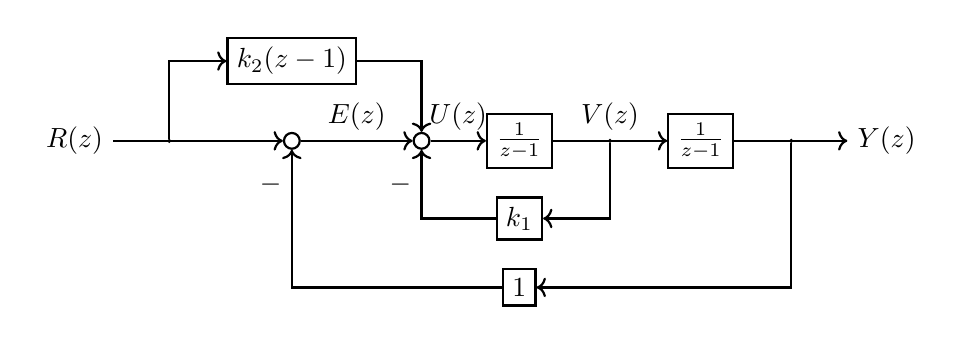
\begin{tikzpicture}[scale=1, thick] 
	\tikzstyle{block} = [draw,rectangle,thick,minimum height=1em,minimum width=1em]
	\tikzstyle{sum} = [draw,circle,inner sep=0mm,minimum size=2mm]
	\tikzstyle{branch} = [draw,circle,fill,inner sep=0pt,minimum size=0.5pt]
	\tikzstyle{connector} = [->,thick]
	\matrix[ampersand replacement=\&, row sep=1em, column sep=2em]{
		\& \&  \node[block](gr){$k_2(z-1)$};\\
		\node(r){$R(z)$};\&\node[branch](br){};\&\node[sum](pe){};\& \node[sum](pu){};\&\node[block](guv){$\frac{1}{z-1}$};\&\node[branch](bv){};\&\node[block](gvy){$\frac{1}{z-1}$};\&\node[branch](by){};\& \node(c){$Y(z)$}; \\
		
		\& \&\&\& \node[block](k1){$k_1$};\\
		\& \&\&\& \node[block](h){$1$};\\
	};
	
	\draw [connector] (r) -- (pe);
	\draw [connector] (br) |-(gr);
	\draw [connector] (pe) -- node[midway,above] {$E(z)$}(pu);
	\draw [connector] (gr) -|(pu);
	\draw [connector] (pu) -- node[midway,above] {$U(z)$}(guv);
	\draw [connector] (guv) -- node[midway,above] {$V(z)$}(gvy);
	\draw [connector] (gvy) --(c);
	\draw [connector]( bv) |-(k1);
	\draw [connector] (k1) -| node[near end,left] {$-$} (pu);
	\draw [connector] (by) |-(h);
	\draw [connector] (h) -| node[very near end,left] {$-$} (pe);
	\end{tikzpicture} 
	
	由梅森公式,得:
	\begin{align*}
	G(z) &=\frac{\frac{k_2}{z-1}+\frac{1}{(z-1)^2}}{1+\frac{k_1}{z-1}+\frac{1}{(z-1)^2}} \\
	&=\frac{1+k_2 (z-1)}{(z-1)^2+(z-1) k_1+1}\\
	&=\frac{k_2 z-k_2+1}{z^2+(k_1-2) z-k_1+2}
	\end{align*}
	
	当系统极点为实数时,满足 $\sigma\%=0$, 其中具有重极点时调节时间最小,因此
	
	\begin{align*}
	(k_1-2)^2 &=4(2-k_1) \\
	k_1 &=\pm 2
	\end{align*}
	舍去 $k_1=-2$(不稳定),得:$k_1=2$ 。
	
	零初始条件下, $r(n)=n,R(z)=\frac{z^{-1}}{(1-z^{-1})^2}$ 时,
	\begin{align*}
	E(s) &=R(s)-G(s)R(s) \\
	&=\frac{(z-1)^2+(z-1) k_1-(z-1)k_2}{k_2 z-k_2+1}\cdot \frac{z^{-1}}{(1-z^{-1})^2}
	\end{align*}
	判断稳定性:
	\begin{align*}
	\frac{(w+1)^2}{(w-1)^2}+\frac{(w+1)(k_1-2)}{w-1}-k_1+2 &=0 \\
	(w+1)^2+(w+1)(w-1)(k_1-2)-(k_1-2)(w-1)^2 &=0 \\
    w^2+2 (k_1 -1) w-2k_1+5 &=0
	\end{align*}
	当 $1<k_1<\frac{5}{2}$ 时系统稳定,且有:
	\begin{align*}
	\lim_{n\to\infty}e(n) &= \lim_{z\to 1}(z-1)E(z) \\
	&=k_1-k_2
	\end{align*}
	因此,当$1<k_1<\frac{5}{2},k_1=k_2$时可使 $\lim_{n\to\infty}e(n)=0$
}




\question(20分)已知控制系统结构图如下所示,已知 $G_c(s)=1,H(s)=s,G(s)=\frac{1}{s(s+1)^3},N(A)=\frac{1}{A+k}$ , 求使系统稳定、无自振的 $k$ 的范围。



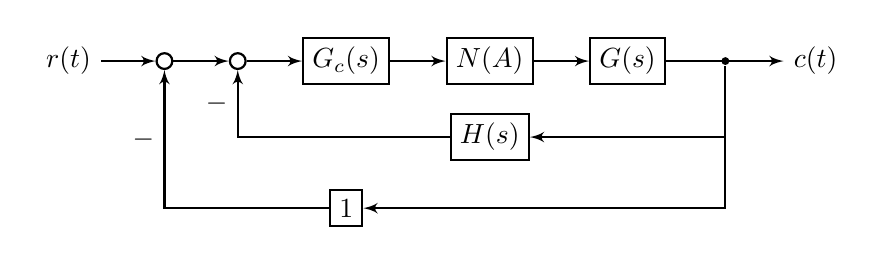
\begin{tikzpicture}[node distance=3em,auto,>=latex', thick]
%\path[use as bounding box] (-1,0) rectangle (10,-2); 
\tikzstyle{block} = [draw,rectangle,thick,minimum height=1em,minimum width=1em]
\tikzstyle{sum} = [draw,circle,inner sep=0mm,minimum size=2mm]
\tikzstyle{branch} = [circle,fill,inner sep=0pt,minimum size=1mm]
\tikzstyle{connector} = [->,thick]

\def\r{\node(r){$r(t)$};}
\def\b(#1){\node[branch](b#1){};}
\def\p(#1){\node[sum](p#1){};}
\def\gc{\node[block](gc){$G_c(s)$};}
\def\na{\node[block](na){$N(A)$};}
\def\gp{\node[block](gp){$G(s)$};}
\def\gh{\node[block](gh){$H(s)$};}
\def\g(#1){\node[block](g#1){$1$};}
\def\c{\node(c){$c(t)$};}

\matrix[ampersand replacement=\&, row sep=1em, column sep=2em]{
	\r  \&  \p(e)  \& \p(r) \& \gc \& \na \& \gp \& \b(c)  \& \c  \\
	\&         \&       \&      \& \gh  \\
	\&         \&       \& \g(h1)    \\
};
\draw [connector](r) -- (pe) ; 
\draw [connector](pe) -- (pr) ; 
\draw [connector](pr)-- (gc) ; 
\draw [connector](gc) -- (na) ; 
\draw [connector](na) -- (gp) ; 
\draw [connector](gp) -- (c) ; 
\draw [connector](bc) |- (gh) ; 
\draw [connector](bc) |- (gh1) ; 
\draw [connector](gh) -| node[near end , left]{$-$} (pr) ; 
\draw [connector](gh1) -| node[near end , left]{$-$} (pe) ; 
\end{tikzpicture} 

\onlyanswer
{
答:系统等效开环传递函数为:
\begin{align*}
G(s) &=\frac{1}{s(s+1)^2}
\end{align*}

计算Nyquist曲线与虚轴交点:
\begin{align*}
\omega_x &=1 \\
G(\omega_x) &= -\frac{1}{2}
\end{align*}
Nyquist曲线不包围负倒描述函数或与其相交:
\begin{align*}
-\frac{1}{N(A)} &< -\frac{1}{2} ,A\in(0,\infty)\\
-A-k&<-\frac{1}{2}\\
k &>\frac{1}{2}
\end{align*}
}

%-------------------------------------------------------
\clearpage

\end{document}
